\section{Methodology}
\label{section:methodology}
This section presents a comprehensive methodological framework for detecting cyberattacks in \gls{evse} networks through federated learning. The approach addresses the critical challenge of achieving high detection accuracy while preserving data privacy in distributed electric vehicle charging infrastructure. The methodology encompasses four integrated components designed to address the unique characteristics of \gls{evse} network environments. These components include advanced data preprocessing with controlled synthetic oversampling, temporal deep learning architecture design, federated learning orchestration, and anomaly detection mechanisms. The framework specifically addresses severe class imbalance in cybersecurity datasets, complex temporal dependencies in attack patterns, and operational requirements for distributed deployment across multiple charging point operators. \\

The methodology introduces three primary innovations for electric vehicle charging network cybersecurity. First, controlled synthetic data generation prevents model degradation through a refined SMOTE implementation that avoids exponential growth of synthetic samples. Second, a temporal network architecture optimized for attack pattern recognition utilizes our proposed \gls{tcn} design with dilated causal convolutions, residual connections, and attention mechanisms. Third, parallel training systems enable quantitative assessment of privacy-utility trade-offs through comprehensive evaluation in both centralized and federated environments. \\

The \gls{tcn} architecture addresses the temporal characteristics of cyber attacks in \gls{ev} charging environments through a carefully designed sequence of dilated causal convolutions. The architecture incorporates batch normalization and Xavier initialization to ensure stable training dynamics across distributed clients. This design specifically targets the complex temporal dependencies inherent in cybersecurity data while maintaining computational efficiency for real-time deployment. The federated learning component implements an efficient federated averaging protocol that maintains model performance while preserving data locality. The implementation partitions datasets across five simulated clients using stratified sampling to maintain class distributions. Each client performs local training for configurable epochs before contributing to global model updates. This approach demonstrates resilience to non-IID data distributions that naturally arise from geographical and operational differences between \gls{evse} deployments. \\

The incorporation of Isolation Forest anomaly detection provides an additional security layer by identifying novel attack patterns that may not conform to known signatures. This component enhances the overall detection capability by addressing zero-day attacks and emerging threat vectors specific to electric vehicle charging infrastructure.

\newpage
\subsection{Hardware and Software Requirements}
The proposed methodology requires specific computational resources for effective deployment. The minimum hardware configuration includes an GPU with 8GB, a multi-core processor with 16 cores, and 16GB RAM. A high-speed solid-state drive is essential for efficient data preprocessing. Federated learning implementations require each client to have 8GB GPU memory for local training tasks. The software implementation utilizes PyTorch framework as the core development platform, with NumPy for numerical operations and Pandas for data manipulation. Scikit-learn handles preprocessing and evaluation metrics, while Plotly provides visualization capabilities.

\subsection{Dataset and Preprocessing}
\label{subsection:dataset}
The CICEVSE2024 dataset constitutes a comprehensive collection of network traffic data from {\acrfull{evse}} systems, specifically developed to advance cybersecurity research in electric vehicle charging infrastructure \cite{cicevse2024}.
%The dataset encompasses 57 individual CSV files distributed across two distinct systems: 28 files from \gls{evse}-A and 29 files from \gls{evse}-B, capturing both benign operational traffic and diverse malicious attack scenarios.
This study utilizes the EVSE-B HPC, and Kernel Events dataset from the CICEVSE2024 collection, which contains network traffic and kernel event data from high-performance computing (HPC) enabled electric vehicle supply equipment under various attack scenarios. The initial dataset, comprising 82 columns, underwent a rigorous preprocessing pipeline to address significant class imbalance and data quality issues. The process began by filtering out non-informative columns and records without valid 'attack' or 'benign' labels. Attack variants were then consolidated into four primary categories: Benign, Cryptojacking, Reconnaissance, and Denial-of-Service (DoS). Problematic features, such as those with constant values, over 95\% missing data, or duplicate columns, were removed.

\begin{figure}[H]
	\centering
	\begin{subfigure}[b]{0.4\textwidth}
		\centering
		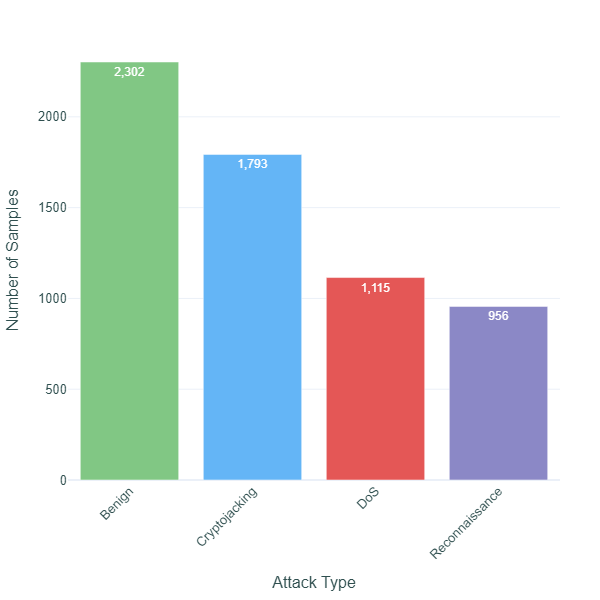
\includegraphics[width=\textwidth]{attack_types.png}
		\caption{Attack Types}
		\label{figure:attack-types}
	\end{subfigure}
	\hspace{0.25cm} 
	\begin{subfigure}[b]{0.4\textwidth}
		\centering
		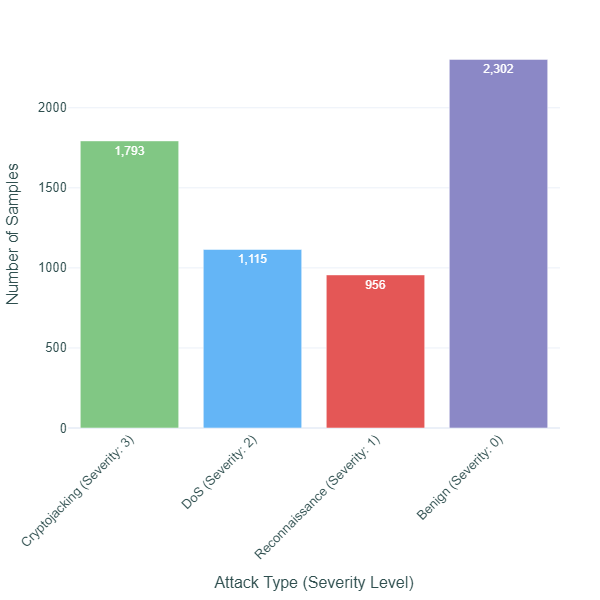
\includegraphics[width=\textwidth]{attack_severity.png}
		\caption{Attack Severity}
		\label{figure:attack-severity}
	\end{subfigure}
	
	\caption{This is the main caption for both images.}
	\label{figure:attacks}
\end{figure}



%Both \gls{evse}-A and \gls{evse}-B systems were monitored during charging and idle operational states, with the systems subjected to multiple attack vectors including aggressive scanning, ICMP-based attacks, operating system fingerprinting, port scanning, push-ACK flooding, service detection, SlowLoris attacks, SYN flooding, TCP and UDP flooding, and vulnerability assessments. The \gls{evse}-B dataset additionally includes data from malicious electric vehicle interactions, providing insights into insider threat scenarios within the \gls{evse} ecosystem. \\

%The research implements a systematic data preprocessing methodology addressing critical challenges in network traffic analysis through multi-stage processing. The framework incorporates automatic detection mechanisms for headers, data types, and encoding formats, while implementing metadata extraction protocols that derive attack classifications from filename conventions. Data quality enhancement procedures include median-based missing value imputation, infinite value conversion, and comprehensive data type standardization. Feature optimization employs zero-variance elimination and correlation analysis with a 0.95 threshold to reduce computational complexity while preserving essential characteristics. \\

%The dataset supports both detailed attack analysis through fifteen distinct categories and binary anomaly detection classification. Feature selection combines F-test scoring, mutual information analysis, and Random Forest-based importance ranking to identify relevant features for attack classification. The resulting preprocessed dataset provides a robust foundation for machine learning applications in electric vehicle supply equipment cybersecurity research, supporting both academic investigation and practical security solution development while maintaining analytical integrity.
%--------------------------------------------------------------
%The study uses comprehensive datasets containing both benign and malicious traffic, structured for three distinct detection models: a binary classifier to distinguish between normal and attack activity, a multiclass classifier to identify specific types of attacks, and a scenario-based model for context-aware threat detection. The raw data consists of diverse network features, including packet-level details and flow statistics, which are essential for identifying anomalous behavior.

%To prepare the data for deep learning analysis, a rigorous multi-stage preprocessing pipeline is employed. The initial stage involves feature selection, where a filtering mechanism validates and retains only informative features by removing those with no variance, single unique values, or an excessive number of missing entries (over 95\%). Following this, a data cleaning and normalization stage handles numerical instabilities by replacing invalid values like 'Not a Number' (NaN) and infinities with zero. The data is then standardized to ensure all features contribute equally to the model's training. The final stage transforms the cleaned data into temporal sequences using a sliding window approach, which captures the time-dependent patterns crucial for identifying network attacks that unfold over time.

%Remaining missing values were handled using median imputation for numeric features and mode imputation for categorical ones. Outliers were identified and removed using the Interquartile Range (IQR) method, which improved the signal-to-noise ratio by trimming 10-15\% of the samples. To counteract severe class imbalance, distinct oversampling techniques were applied: Random Oversampling was used to achieve a 1:1 ratio for binary classification, while SMOTE and ADASYN were employed for the more complex multi-class and scenario-based classification tasks, respectively. This comprehensive preprocessing resulted in three specialized, analysis-ready datasets tailored for binary, multi-class, and scenario-based attack detection.

The preprocessing pipeline follows a modular, five-stage architecture that emphasizes data quality over quantity. The system begins with data ingestion and exploration, followed by comprehensive data cleaning that removes non-informative features and validates record consistency. The pipeline then applies advanced feature engineering techniques, including outlier detection using Interquartile Range methodology and correlation-based feature importance analysis. To address the common challenge of class imbalance in cybersecurity data, the system implements multiple balancing strategies including \gls{smote} and \gls{adasyn} with fallback mechanisms. \\

The framework generates three specialized datasets tailored for different operational security scenarios: binary classification for basic attack detection, multi-class classification for specific attack type identification, and scenario-based classification for strategic threat analysis. Each dataset maintains consistent feature representations while optimizing target variable encodings for their specific classification objectives. The implementation addresses critical cybersecurity data analysis challenges including temporal data leakage prevention, categorical variable standardization, and statistical property preservation throughout preprocessing operations. %The pipeline's emphasis on transparency, reproducibility, and rigorous quality assurance standards provides a robust foundation for developing production-ready cybersecurity machine learning systems capable of effectively detecting and classifying network-based threats in electric vehicle charging infrastructure environments.

\subsection{Proposed Model Architecture}
\label{subsection:proposed-model-architecture}
Our proposed framework employs an Advanced Temporal Convolutional Network (AdvancedTCN) architecture that significantly extends traditional TCN designs through the integration of multi-head attention mechanisms and enhanced regularization strategies. The architecture is specifically engineered to capture complex temporal dependencies in EVSE network traffic while maintaining computational efficiency for real-time deployment.
The core architecture consists of three hierarchical temporal blocks with progressively increasing channel dimensions {64, 128, 256}, enabling the network to learn increasingly abstract representations of network behavior. Each temporal block implements a sophisticated residual structure with two convolutional layers, batch normalization, and dropout regularization. The use of Xavier uniform initialization ensures stable gradient flow from the network's inception, addressing the vanishing gradient problem common in deep temporal architectures.

\subsubsection{Temporal Convolutional Network}

% Preamble must include: \usepackage{booktabs}

% Preamble must include:
% \usepackage{tabularx}
% \usepackage{booktabs}

% Preamble must include: \usepackage{booktabs}
\begin{table}[h!]
	\centering
	% --- Commands to add padding ---
	\renewcommand{\arraystretch}{1.4} % Increase vertical space
	\setlength{\tabcolsep}{12pt}      % Increase horizontal space
	% -----------------------------
	\caption{Enhanced architectural components and their configurations.}
	\label{tab:arch_components_enhanced}
	\begin{tabular}{ll}
		\toprule
		\textbf{Component} & \textbf{Configuration} \\
		\midrule
		Temporal Blocks & 3 layers, \{64, 128, 256\} channels \\
		Kernel Size & 5 \\
		Dilation Pattern & \{1, 2, 4\} \\
		Attention Mechanism & 8 heads, $d_{\text{model}}$=256 \\
		Batch Normalization & After each convolution \\
		Dropout Rates & \{0.3, 0.5\} \\
		Activation & ReLU \\
		Output Architecture & 3-layer MLP with BatchNorm \\
		\bottomrule
	\end{tabular}
\end{table}

Table~\ref{tab:arch_components_enhanced} summarizes the key architectural components of our enhanced model. The temporal blocks employ a hierarchical structure with three layers containing 64, 128, and 256 channels respectively, enabling progressive feature extraction from low-level patterns to high-level representations. The kernel size of 5 provides extended local pattern detection capabilities, while the dilation pattern of \{1, 2, 4\} ensures multi-scale temporal coverage by capturing dependencies at different time scales. The attention mechanism utilizes 8 heads with a model dimension of 256 to enable dynamic feature focusing on the most relevant temporal patterns. Batch normalization is applied after each convolution to maintain training stability and accelerate convergence. A hierarchical dropout strategy with rates of 0.3 and 0.5 provides regularization at different network depths to prevent overfitting. ReLU activation functions introduce non-linear transformations throughout the network, while the output architecture employs a robust 3-layer MLP with batch normalization for reliable classification performance. \\


The multi-head attention mechanism represents a significant advancement over traditional TCN architectures. Following the temporal convolution layers, the network applies 8-head self-attention to the temporal dimension, enabling dynamic weighting of different time steps based on their relevance to the classification task. The attention mechanism computes:

\begin{equation}
	\text{Attention}(Q, K, V) = \text{Softmax}\left(\frac{QK^T}{\sqrt{d_k}}\right) \cdot V
	\label{eq:attention}
\end{equation}

where $Q$, $K$, and $V$ represent the query, key, and value projections of the input features, and \( d_k \)​ is the dimension of each attention head. This mechanism allows the model to learn long-range dependencies and focus on critical temporal segments that may indicate attack patterns. The classifier head employs a three-layer fully connected architecture with progressive dimension reduction {256 $\rightarrow$ 128 $\rightarrow$ $classes$}. Each hidden layer incorporates batch normalization and dropout, with dropout rates of 0.5 and 0.3 respectively, providing robust regularization against overfitting. The use of adaptive average pooling before the classifier ensures consistent input dimensions regardless of sequence length variations. \\


\subsubsection{Federated Learning}
Our federated learning implementation represents a comprehensive framework for distributed model training that preserves data privacy while maintaining detection performance. The framework implements an efficient federated averaging protocol with support for heterogeneous client configurations and adaptive local training strategies. The client architecture encapsulates local model training within isolated environments, ensuring data never leaves the client's domain. Each FederatedClient maintains a deep copy of the global model, preventing interference between clients during parallel training. The local training process employs the Adam optimizer with a learning rate of 0.001, chosen for its adaptive learning rate properties that accommodate varying data distributions across clients. The federated learning configuration is detailed in Table \ref{tab:fedlearn_config}.

\begin{table}[h]
	\centering
	\renewcommand{\arraystretch}{1.4} % Increase vertical space
	\setlength{\tabcolsep}{12pt}      % Increase horizontal space
	\caption{Federated learning configuration}
	\label{tab:fedlearn_config}
	\begin{tabular}{ll}
		\toprule
		\textbf{Parameter} & \textbf{Value} \\
		\midrule
		Number of Clients & 5 \\
		Communication Rounds & 5 \\
		Local Epochs per Round & 1 \\
		Batch Size & 64 \\
		Client Data Distribution & Stratified random split \\
		Aggregation Method & Weighted FedAvg \\
		\bottomrule
	\end{tabular}
\end{table}

The number of clients, set at 5, represents the regional EVSE operators involved in the federated learning process. The communication rounds, established at 5, are designed to balance convergence and communication efficiency effectively. Local epochs per round, limited to 1, are implemented to prevent client overfitting and ensure model generalization. The batch size, fixed at 64, optimizes memory usage during training. The client data distribution, configured as a stratified random split, maintains class balance across the dataset. Lastly, the aggregation method, utilizing Weighted FedAvg, accounts for floating-point parameters to enhance the accuracy of the aggregated model.

The global model update is defined as follows:

\begin{equation}
	w_{\text{global}}^{(t+1)} = \frac{1}{K} \sum_{k=1}^{K} w_k^{(t+1)}
\end{equation}

where \( w_k^{(t+1)} \) represents the updated weights from client \( k \) after local training in round \( t+1 \), and \( K \) is the number of participating clients. \\

%-------------------------------------------------------------------------------------------------------------------------------
The \acrlong{fl} implementation enables privacy-preserving collaborative training across multiple \gls{evse} operators without requiring data centralization. This approach fundamentally transforms how security intelligence is shared across critical infrastructure networks by allowing participants to contribute to model improvement while maintaining complete control over their sensitive operational data. \\

The \gls{fl} protocol operates through structured iterative rounds that combine local training phases with global model aggregation. Each communication round involves careful coordination between a central aggregation server and selected client participants. The protocol ensures that raw data never leaves individual operator premises while enabling the development of robust global models that benefit from diverse threat patterns observed across multiple networks. \\

%\section{Federated Learning Protocol}
The main federated learning protocol coordinates the training process across distributed \gls{evse} operators as presented in~\reference{algorithm:federated-learning}. The protocol begins with initialization of global model parameters using standard random initialization techniques appropriate for deep neural networks. During each communication round, the system selects a subset of available clients to participate in training, which provides flexibility for operators with varying computational resources or availability constraints. \\

\begin{algorithm}[H]
	\caption{Federated Learning for EVSE Intrusion Detection~\vspace{0.25em}}
	\label{algorithm:federated-learning}
	\vspace*{3.5pt}
	{
		\setstretch{1.25}
		\SetAlgoNlRelativeSize{-1} % Adjust the size of the line numbers
		\IncMargin{1em} % Increase the margin for the line numbers
		\KwIn{Global model $\theta_0$, $K$ clients, $T$ rounds, $E$ local epochs}
		\KwOut{Trained global model $\theta_T$}
		Initialize global model $\theta_0$\;
		\For{round $t = 1$ \KwTo $T$}{
			$S_t \leftarrow$ sample subset of $K$ clients\;
			\ForPar{each client $k \in S_t$}{
				$\theta^k_{t+1} \leftarrow$ \textsc{ClientUpdate}($k$, $\theta_t$)\;
			}
			$\theta_{t+1} \leftarrow$ \textsc{FederatedAverage}($\{\theta^k_{t+1}\}_{k \in S_t}$)\;
		}
		\Return{$\theta_T$}\;
	}
\end{algorithm}
\medskip

The parallel execution of client training ensures efficient utilization of distributed computational resources while maintaining privacy boundaries. In each communication round, selected clients receive the current global model parameters and perform local training on their private data for a specified number of epochs. After local training, clients send their updated model parameters back to the central server, which aggregates them to create an improved global model. \\

%\section{Client Update Process}
The client training process implements local stochastic gradient descent optimization using each operator's private dataset as detailed in \reference{algorithm:client-update}. The local training process ensures that each client performs multiple epochs of optimization on their private data before sharing parameter updates. This approach reduces communication overhead while allowing sufficient local adaptation to each operator's specific network characteristics and threat patterns. \\

\begin{algorithm}[H]
	\caption{Client Update Function\vspace{0.25em}}
	\label{algorithm:client-update}
	\vspace*{3.5pt}
	{
		\setstretch{1.25}
		\SetAlgoNlRelativeSize{-1} % Adjust the size of the line numbers
		\KwIn{Client $k$, global parameters $\theta$}
		\KwOut{Updated local parameters $\theta$}
		$B \leftarrow$ split local data into batches\;
		$\theta \leftarrow \theta$ \tcp{Copy global parameters}
		\For{epoch $i = 1$ \KwTo $E$}{
			\For{batch $b \in B$}{
				$\theta \leftarrow \theta - \eta\nabla\ell(\theta; b)$\;
			}
		}
		\Return{$\theta$}\;
	}
\end{algorithm}

The algorithm maintains standard stochastic gradient descent principles while operating within the federated learning constraint that data cannot be shared between participants. The implementation computes gradients only on locally available data, ensuring that sensitive network traffic information remains within each operator's premises.
%\section{Privacy and Security Benefits}
This federated learning approach addresses the critical challenge of improving detection capabilities while maintaining data confidentiality. Operators can benefit from collective intelligence without sharing sensitive network traffic data, enabling the development of more robust intrusion detection systems that leverage diverse threat patterns from multiple \gls{evse} networks while preserving individual operator privacy and data sovereignty. \\

%\subsection{Federated Temporal Block Training}
%\label{subsec:federated_temporal_training}
The integration of temporal blocks within the federated learning framework requires careful consideration of computational complexity and communication efficiency. Each client must train the complete temporal block architecture on their local data while maintaining synchronization with the global model updates. The local training objective for client $k$ with temporal blocks is expressed in \reference{equation:local-objective}.

\begin{equation}
	\label{equation:local-objective}
	\mathcal{L}_k(\theta) = \frac{1}{|\mathcal{D}_k|} \sum_{(\mathbf{x}, y) \in \mathcal{D}_k} \ell(f_{\theta}(\mathbf{x}), y) + \lambda \mathcal{R}(\theta)
\end{equation}

where $f_{\theta}(\mathbf{x})$ represents the output of the temporal block network with parameters $\theta$, $\ell$ denotes the loss function appropriate for the detection task, and $\mathcal{R}(\theta)$ implements regularization to prevent overfitting. The regularization term is particularly important in federated settings where each client may have limited data diversity.

%\subsubsection{Training Methodology}
Training methodology implements parallel strategies for both centralized and federated configurations, enabling direct performance comparison under identical conditions. The training process incorporates advanced optimization techniques and regularization strategies tailored to the characteristics of \gls{evse} network data. For centralized training, we employ a single model trained on the complete dataset. The federated training process distributes the training data across clients with random permutation, ensuring each client receives a representative data sample while maintaining privacy. Each communication round consists of three phases: (\rom{1}) global model distribution to clients, (\rom{2}) local training on private data, and (\rom{3}) aggregation of updated weights. 

\begin{equation}
	\label{equation:binary-loss}
	\mathcal{L}_{binary} = -\frac{1}{N}\sum_{i=1}^{N}[y_i\log(\sigma(\hat{y}_i)) + (1-y_i)\log(1-\sigma(\hat{y}_i))]
\end{equation}

\begin{equation}
	\label{equation:multiclass-loss}
	\mathcal{L}_{multiclass} = -\frac{1}{N}\sum_{i=1}^{N}\sum_{c=1}^{C}y_{i,c}\log(\text{softmax}(\hat{y}_i)_c)
\end{equation}

This process iterates for 5 rounds, with validation performed after each round to monitor convergence. We employ different loss functions tailored to each detection scenario, ensuring optimal training for the specific classification task at hand. For binary intrusion detection, we use binary cross-entropy loss as defined in \reference{equation:binary-loss}, and \reference{equation:multiclass-loss} extends binary cross-entropy to multiple classes, where $C$ represents the total number of attack types. The softmax function normalizes raw outputs into a probability distribution over all classes. The one-hot encoded true labels $y_{i,c}$ ensure that only the loss for the correct class contributes to each sample's total loss.

\subsection{Adaptive Trust-Weighted Federated Aggregation}
\label{subsection:trust-weighted-aggregation}
Traditional federated averaging assigns equal weights to all clients, which can be suboptimal when clients have varying data quality, computational resources, or performance characteristics. We propose an Adaptive Trust-Weighted Federated Aggregation (TWFA) mechanism that dynamically adjusts client contributions based on multiple trust factors. \\

The trust score for client $k$ at round $t$ is computed as a weighted combination of four components:

\begin{equation}
	\label{equation:trust-score}
	\tau_k^{(t)} = \alpha_1 \cdot \tau_{perf}^k + \alpha_2 \cdot \tau_{data}^k + \alpha_3 \cdot \tau_{hist}^k + \alpha_4 \cdot \tau_{loss}^k
\end{equation}

where $\tau_{perf}^k$ represents performance trust based on validation accuracy, $\tau_{data}^k$ captures data quality trust based on sample size and distribution, $\tau_{hist}^k$ incorporates historical trust using exponential moving average, and $\tau_{loss}^k$ reflects training quality based on loss convergence. The coefficients $\{\alpha_1, \alpha_2, \alpha_3, \alpha_4\}$ are set to $\{0.4, 0.2, 0.3, 0.1\}$ to prioritize validation performance and historical reliability. \\

The weighted global model update becomes:

\begin{equation}
	\label{equation:trust-weighted-update}
	w_{\text{global}}^{(t+1)} = \frac{\sum_{k=1}^{K} \tau_k^{(t)} \cdot w_k^{(t+1)}}{\sum_{k=1}^{K} \tau_k^{(t)}}
\end{equation}

Historical trust is updated using exponential moving average with momentum $\beta = 0.7$:

\begin{equation}
	\label{equation:historical-trust}
	\tau_{hist}^{k,(t+1)} = \beta \cdot \tau_{hist}^{k,(t)} + (1 - \beta) \cdot \tau_{perf}^{k,(t)}
\end{equation}

This adaptive mechanism ensures that high-performing clients with consistent performance history have greater influence on the global model, while underperforming or unstable clients contribute less, improving overall convergence and robustness. The complete algorithm is presented in \reference{algorithm:trust-weighted-aggregation}.

\begin{algorithm}[H]
	\caption{Adaptive Trust-Weighted Federated Aggregation\vspace{0.25em}}
	\label{algorithm:trust-weighted-aggregation}
	\vspace*{3.5pt}
	{
		\setstretch{1.25}
		\SetAlgoNlRelativeSize{-1}
		\KwIn{Client models $\{w_k\}_{k=1}^K$, metrics $\{\mathcal{M}_k\}_{k=1}^K$, historical trust $\{\tau_{hist}^k\}$}
		\KwOut{Aggregated global model $w_{global}$, updated trust scores}

		\For{each client $k = 1$ \KwTo $K$}{
			$\tau_{perf}^k \leftarrow \mathcal{M}_k[\text{val\_accuracy}]$\;
			$\tau_{data}^k \leftarrow \text{normalize}(\mathcal{M}_k[\text{num\_samples}])$\;
			$\tau_{loss}^k \leftarrow 1 - \text{normalize}(\mathcal{M}_k[\text{val\_loss}])$\;
			$\tau_k \leftarrow 0.4 \cdot \tau_{perf}^k + 0.2 \cdot \tau_{data}^k + 0.3 \cdot \tau_{hist}^k + 0.1 \cdot \tau_{loss}^k$\;
			$\tau_{hist}^k \leftarrow 0.7 \cdot \tau_{hist}^k + 0.3 \cdot \tau_{perf}^k$ \tcp{Update historical trust}
		}

		$w_{global} \leftarrow \frac{\sum_{k=1}^K \tau_k \cdot w_k}{\sum_{k=1}^K \tau_k}$ \tcp{Weighted aggregation}

		\Return{$w_{global}$, $\{\tau_{hist}^k\}$}\;
	}
\end{algorithm}

\subsection{Hierarchical Multi-Resolution Temporal Attention}
\label{subsection:multi-resolution-attention}
Attack patterns in EVSE networks manifest at different temporal scales: DoS attacks exhibit short-term burst patterns (seconds), cryptojacking shows medium-term resource consumption patterns (minutes), and reconnaissance displays long-term scanning patterns (hours). Traditional single-scale attention mechanisms fail to capture this multi-scale temporal structure. \\

We propose a Hierarchical Multi-Resolution Temporal Attention (AMRTA) mechanism that applies parallel attention at multiple temporal resolutions $\mathcal{S} = \{1, 5, 15, 30\}$ time steps, corresponding to immediate, short-term, medium-term, and long-term dependencies:

\begin{equation}
	\label{equation:multi-resolution-attention}
	\mathbf{h}_{\text{multi}} = \sum_{s \in \mathcal{S}} \lambda_s \cdot \text{Attention}_s(Q_s, K_s, V_s)
\end{equation}

where $\text{Attention}_s$ operates on temporal windows of scale $s$, and $\lambda_s$ are learnable scale fusion weights initialized uniformly. Each scale-specific attention head captures dependencies at its corresponding temporal resolution:

\begin{equation}
	\label{equation:scale-specific-attention}
	\text{Attention}_s(Q_s, K_s, V_s) = \text{Softmax}\left(\frac{Q_s K_s^T}{\sqrt{d_k}}\right) V_s
\end{equation}

The queries, keys, and values for each scale are computed by applying average pooling with stride $s$ to the input sequence:

\begin{equation}
	\label{equation:scale-pooling}
	\mathbf{x}_s = \text{AvgPool}(\mathbf{x}, \text{stride}=s)
\end{equation}

This hierarchical design enables the model to simultaneously attend to immediate packet-level anomalies and long-term behavioral patterns, significantly improving detection of complex multi-stage attacks. The architecture employs 8 attention heads per scale with $d_{model} = 256$, and the scale fusion weights are learned end-to-end during training.

\subsection{Federated Concept Drift Detection}
\label{subsection:concept-drift-detection}
Real-world EVSE networks experience concept drift as attack patterns evolve over time. Static models trained on historical data degrade in performance when confronted with novel attack variants or changing network conditions. We implement a Federated Concept Drift Detection system using the ADWIN (Adaptive Windowing) algorithm to identify significant changes in error distribution. \\

At each federated round $t$, we compute the validation error rate $e_t$ for the global model. ADWIN maintains a sliding window of recent error rates and detects drift when the difference between sub-window means exceeds a threshold:

\begin{equation}
	\label{equation:drift-detection}
	|\mu_{recent} - \mu_{historical}| > \epsilon_{cut} = \sqrt{\frac{1}{2m} \cdot \ln\frac{4N^2}{\delta}}
\end{equation}

where $m$ is the harmonic mean of sub-window sizes, $N$ is the total window size, and $\delta$ is the confidence parameter. When drift is detected, the system triggers adaptive responses:

\begin{equation}
	\label{equation:adaptive-lr}
	\eta^{(t+1)} =
	\begin{cases}
		5 \cdot \eta_0 & \text{if major drift detected} \\
		2 \cdot \eta_0 & \text{if warning detected} \\
		\eta_0 & \text{otherwise}
	\end{cases}
\end{equation}

where $\eta_0$ is the base learning rate. This adaptive learning rate mechanism accelerates model adaptation during drift periods while maintaining stable training otherwise. The drift detector operates at the global level, analyzing aggregated performance metrics across all clients to identify systemic changes in the threat landscape rather than client-specific fluctuations.

\subsection{Byzantine-Resilient Aggregation}
\label{subsection:byzantine-resilience}
Federated learning systems are vulnerable to Byzantine attacks where malicious or compromised clients submit corrupted model updates to degrade global model performance or inject backdoors. To defend against such threats, we integrate the Krum aggregation algorithm, which selects the most representative client update based on geometric proximity in parameter space. \\

Given $K$ client updates $\{w_k\}_{k=1}^K$, Krum computes pairwise distances and selects the client whose update is closest to the majority:

\begin{equation}
	\label{equation:krum-score}
	\text{Score}(w_i) = \sum_{j \in \mathcal{N}_i} \|w_i - w_j\|^2
\end{equation}

where $\mathcal{N}_i$ contains the $K - f - 2$ nearest neighbors of client $i$, and $f$ is the maximum number of Byzantine clients tolerated. The client with the minimum score is selected:

\begin{equation}
	\label{equation:krum-selection}
	w_{\text{global}}^{(t+1)} = w_{\arg\min_i \text{Score}(w_i)}
\end{equation}

For enhanced robustness, we implement Multi-Krum which averages the $m$ clients with lowest Krum scores:

\begin{equation}
	\label{equation:multi-krum}
	w_{\text{global}}^{(t+1)} = \frac{1}{m} \sum_{i \in \mathcal{K}_m} w_i
\end{equation}

where $\mathcal{K}_m$ contains the $m$ clients with lowest Krum scores. In our implementation, we set $f = 1$ (tolerating up to 30\% malicious clients with $K=5$) and $m = 3$ for Multi-Krum. This defense mechanism operates transparently during federated aggregation, requiring no modification to client-side training procedures.

\subsection{Federated SHAP Explainability}
\label{subsection:federated-shap}
Explainability is critical for operational deployment of intrusion detection systems, enabling security analysts to understand model decisions and identify root causes of detected threats. However, traditional SHAP (SHapley Additive exPlanations) requires access to raw data, conflicting with federated learning's privacy guarantees. We present the first Federated SHAP framework for intrusion detection that computes local SHAP values at each client and aggregates them without raw data sharing. \\

For each client $k$, we compute GradientSHAP attributions for test samples $\mathbf{x}_i$:

\begin{equation}
	\label{equation:gradient-shap}
	\phi_j^k(\mathbf{x}_i) = \mathbb{E}_{\mathbf{x}' \sim \mathcal{D}_k}\left[\frac{\partial f(\mathbf{x}')}{\partial x_j'} \cdot (x_{ij} - x_{ij}')\right]
\end{equation}

where $\phi_j^k$ is the SHAP value for feature $j$ at client $k$, $\mathcal{D}_k$ is the client's local data distribution, and $f$ is the model output. We aggregate SHAP values across samples and time steps to obtain client-level feature importance:

\begin{equation}
	\label{equation:local-importance}
	I_j^k = \frac{1}{N_k T} \sum_{i=1}^{N_k} \sum_{t=1}^{T} |\phi_j^k(\mathbf{x}_i^t)|
\end{equation}

where $N_k$ is the number of samples at client $k$ and $T$ is the sequence length. Global feature importance is computed via trust-weighted aggregation:

\begin{equation}
	\label{equation:global-importance}
	I_j^{global} = \frac{\sum_{k=1}^K \tau_k \cdot I_j^k}{\sum_{k=1}^K \tau_k}
\end{equation}

This federated explainability framework enables security analysts to identify the most critical features for attack detection (e.g., packet rates, connection patterns, resource consumption) without accessing individual operator data. The framework also computes per-attack-class feature importance, revealing that DoS attacks are primarily characterized by network-level features, while cryptojacking detection relies heavily on kernel-level resource metrics.

\subsection{Evaluation Metrics}
\label{subsection:evaluation-metrics}
The evaluation of intrusion detection systems in EVSE networks requires a comprehensive set of metrics that capture different aspects of model performance. Given the severe class imbalance inherent in our dataset, where attack samples represent a small fraction of total network traffic, relying on a single metric would provide an incomplete and potentially misleading assessment of detection capabilities. Our evaluation framework employs six complementary metrics that collectively quantify the model's ability to correctly identify attacks while minimizing false alarms—a critical balance for operational deployment in production environments. \\

%The selection of these metrics is guided by the specific requirements of EVSE security operations. In this context, the cost of missing an attack (false negative) could result in service disruption, financial losses, or compromise of critical infrastructure, while excessive false alarms (false positives) could overwhelm security teams and erode trust in the automated detection system. Therefore, our evaluation framework emphasizes metrics that provide nuanced insights into these different failure modes, enabling informed decisions about operational thresholds and deployment strategies.

%**Accuracy** gives a general overview but is unreliable in imbalanced datasets. **Recall** (or sensitivity) is critical as it measures the model's ability to identify all actual attacks. **Precision** complements recall by measuring the reliability of the alarms that are raised. The **F1 Score** provides a balanced measure by calculating the harmonic mean of precision and recall, making it a primary metric for imbalanced data. The **False Positive Rate (FPR)** specifically quantifies the rate of false alarms, which directly impacts security team workload. Finally, the **Area Under the Curve (AUC)** offers a threshold-independent evaluation of the model's ability to distinguish between malicious and benign traffic.



%The performance of the intrusion detection system is quantified using the following metrics, where $TP$ is True Positives, $TN$ is True Negatives, $FP$ is False Positives, and $FN$ is False Negatives.

Our comprehensive evaluation framework employs 20 distinct visualization techniques and multiple quantitative metrics to assess model performance from various perspectives. The framework is designed to provide actionable insights for security analysts while enabling rigorous comparison between centralized and federated approaches.
Core Performance Metrics: We evaluate models using accuracy, precision, recall, F1-score, and AUC-ROC for threshold-independent assessment. For multiclass scenarios, we compute both macro and weighted averages to account for class imbalance. The evaluation function efficiently processes test data in batches of 256 samples, optimizing memory usage while maintaining numerical precision.

\begin{equation}
	\text{Accuracy} = \frac{TP + TN}{TP + TN + FP + FN}
	\label{eq:accuracy}
\end{equation}

\begin{equation}
	\text{Recall} = \frac{TP}{TP + FN}
	\label{eq:recall}
\end{equation}

\begin{equation}
	\text{Precision} = \frac{TP}{TP + FP}
	\label{eq:precision}
\end{equation}

\begin{equation}
	\text{F1 Score} = 2 \times \frac{\text{Precision} \times \text{Recall}}{\text{Precision} + \text{Recall}}
	\label{eq:f1_score}
\end{equation}

\begin{equation}
	\text{FPR} = \frac{FP}{FP + TN}
	\label{eq:fpr}
\end{equation}

\begin{equation}
	\text{AUC} = \sum_{i=1}^{n} \frac{(\text{TPR}_i + \text{TPR}_{i-1})}{2} \cdot (\text{FPR}_i - \text{FPR}_{i-1})
	\label{eq:auc}
\end{equation}